
%\documentclass[./main.tex(path of main file)]{subfiles}
\documentclass[10pt]{article}
\usepackage{amsmath}
\DeclareMathOperator*{\argmin}{arg\,min} % thin space, limits underneath in displays
\DeclareMathOperator*{\argmax}{arg\,max} % thin space, limits underneath in displays
\newtheorem{thm}{Theorem}
\usepackage{amssymb}
\usepackage{amsfonts}
\usepackage{mathrsfs}
\usepackage{bm}
\usepackage{indentfirst}
\setlength{\parindent}{0em}
\usepackage[margin=1in]{geometry}
\usepackage{graphicx}
\usepackage{setspace}
\doublespacing
\usepackage[flushleft]{threeparttable}
\usepackage{booktabs,caption}
\usepackage{float}
\usepackage[sort,comma]{natbib}
\usepackage[hidelinks]{hyperref}
\usepackage{booktabs}
\usepackage{multirow}

\usepackage{import}
\usepackage{xifthen}
\usepackage{pdfpages}
\usepackage{transparent}
\usepackage{subfiles}
\usepackage{blindtext}
\usepackage{glossaries}
\usepackage{pdflscape}
\usepackage{adjustbox}
\usepackage{rotating}
\usepackage{eurosym,geometry,ulem,subcaption,caption,color,sectsty,comment,footmisc,pdflscape,array}

% Format definition list
\newenvironment{mylist}[1]%
  {\begin{list}{}{\settowidth{\labelwidth}{\textbf{#1}}
   \setlength{\leftmargin}{\labelwidth}
   \addtolength{\leftmargin}{\labelsep}
   \renewcommand{\makelabel}[1]{\textbf{\hfill##1}}}}%
  {\end{list}}



\newcommand{\incfig}[1]{%
\def\svgwidth{\columnwidth}
\import{./figures/}{#1.pdf_tex}
}




\title{}
\author{}
\date{}


\begin{document}
\maketitle


\section{Post-Stratification Weights}

\subsection{Intro}

It requires the use of auxiliary information about the population and may take a number of different
variables into account.
Information usually needed:
\begin{itemize}
\item Population estimates of the distribution of a set of demographic
characteristics that have also been measured in the sample
\item For example, information found in the Census (as a measure of population) such as:
		\begin{itemize}
		\item Sex
		\item Age
		\item Education attainment
		\item Household size
		\item Residence
		\item Region
		\end{itemize}
\item Population data for community-based samples:
		\begin{itemize}
		\item US Census tabulations
		\item The Current Population Survey (CPS)
		\item The American Community Survey (ACS)
		\end{itemize}
\end{itemize}


\subsection{Single-variable dataset}

\begin{figure}[H]
\center{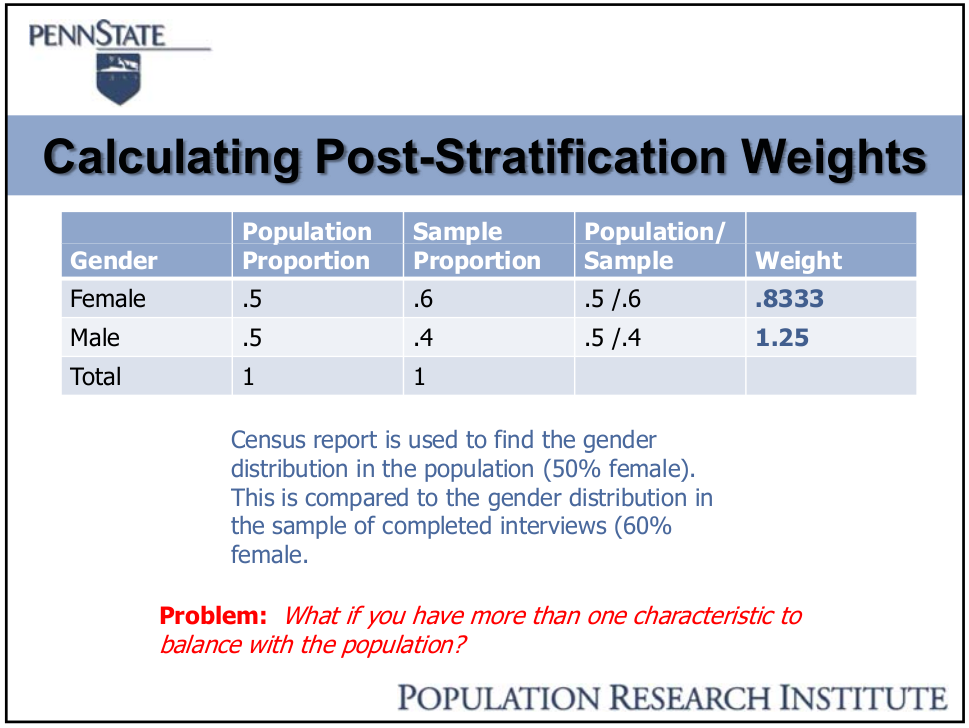
\includegraphics[width = 0.8\textwidth]  {figures/one_variable_weight.png}}
\label{fig:}
\end{figure}


\subsection{Multi-variable dataset}

\begin{figure}[H]
\center{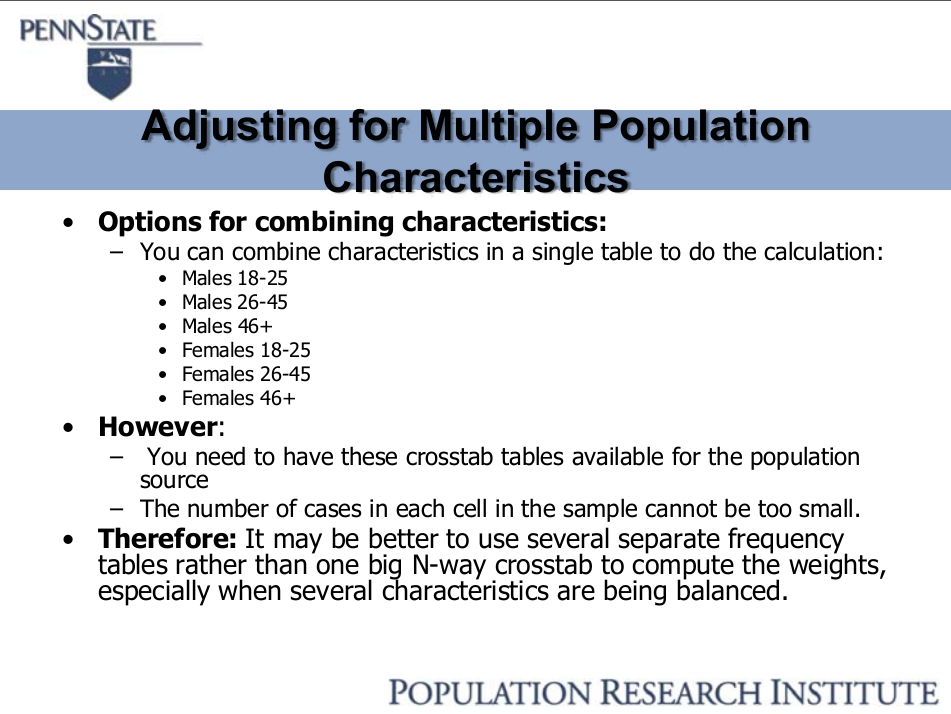
\includegraphics[width = 0.8\textwidth]  {figures/multi_variable_weight.png}}
\label{fig:}
\end{figure}

{\textbf {How to compute the weight given multiple characteristics features?}}

\begin{figure}[H]
\center{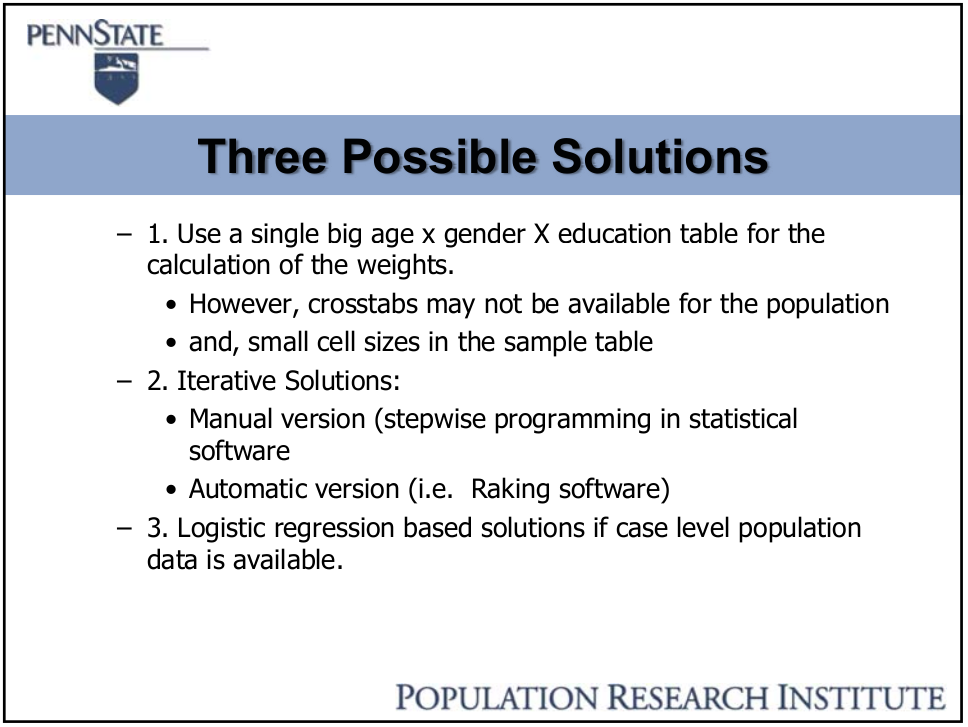
\includegraphics[width = 0.8\textwidth]  {figures/three_ways_of_weight_computing.png}}
\label{fig:}
\end{figure}


\subsection{Method 1: Crosstabs}

Suppose the population and survey data contain two characteristics features, sex and education.
\begin{itemize}
		\item Sex: male (sex = 1), female (sex = 0)
		\item edu: high edu (edu = 1), low edu (edu = 0)
\end{itemize}

Here is an example of the population and survey data
\begin{figure}[H]
\center{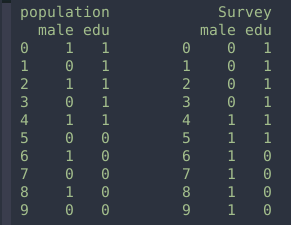
\includegraphics[width = 0.4\textwidth]  {figures/example_population_and_survey.png}}
\label{fig:}
\end{figure}


Hence, we can group obs into four groups
\begin{itemize}
		\item female with low edu (code: 00)
		\item female with high edu (code: 01)
		\item male with low edu (code: 10)
		\item male with high edu (code: 11)
\end{itemize}

Here is the percentage share of each group,
\begin{equation*}
share_{\text{ group }} = \frac{N_{\text{ group }}}{N_{\text{ num. of obs }}}.
\end{equation*}

For example, there are 2 female with high edu, and there are 10 obs. 
Hence $ share_{\text{ female with low edu }} = \frac{2}{10} = 0.2 $

Here is the percentage share for each group in the population and the survey.
\begin{figure}[H]
\center{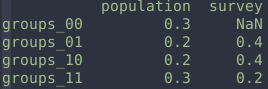
\includegraphics[width = 0.4\textwidth]  {figures/share_of_each_group.png}}
\label{fig:}
\end{figure}

NaN says there is no female with low edu (code: 00) in the survey.

To make the demographic feature in the survey being consistent with the population,
the weight for group g is defined as
\begin{equation}
weight_{g} = \frac{\text{ share in population }_{g}}{\text{ share in survey }_{g}}.
\label{eqn:weight_crosstabs}
\end{equation}

For example, the weight for female with high edu (code: 01) is 
\begin{align*}
weight_{\text{ female with high edu }} &= \frac{\text{ share in population }_{\text{ female with high edu }}}{\text{ share in survey }_{\text{ female with high edu }}}\\
&= \frac{0.2}{0.4}\\
&= 0.5
\end{align*}

Here is the crosstab weights for each group.
\begin{figure}[H]
\center{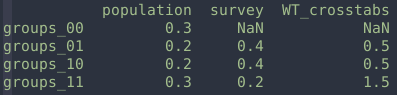
\includegraphics[width = 0.4\textwidth]  {figures/weight_crosstabs.png}}
\label{fig:}
\end{figure}



\subsection{Method 3: Logistic regression}
Given the population and survey data in ``Method 1",

\begin{figure}[H]
\center{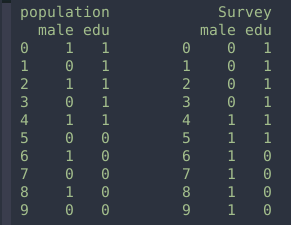
\includegraphics[width = 0.4\textwidth]  {figures/example_population_and_survey.png}}
\label{fig:}
\end{figure}

Add a column called "sample" set to 1 for the survey data, and set to 0 for the population data.
\begin{figure}[H]
\center{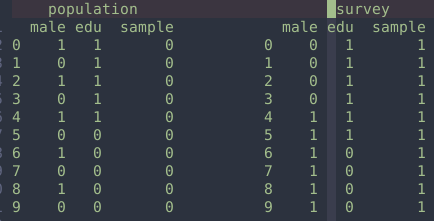
\includegraphics[width = 0.4\textwidth]  {figures/example_population_and_survey_for_method_logit.png}}
\label{fig:}
\end{figure}

Then merge the two dataset vertically. And fit the equation below,
\begin{equation}
sample = \beta_0  +  \beta_1 male  + \beta_2 edu.
\end{equation}

Then get the estimated probability
\begin{equation*}
		Prob(Sample = 1|\bm{x}) = \frac{exp(\bm{x}'\bm{\beta})}{1  +  exp(\bm{x}'\bm{\beta})} = \Lambda(\bm{x}'\bm{\beta}) = p,
\end{equation*}
by calling ``smf.logit().fit().predict()".

The odds is
\begin{equation*}
Odds = \frac{Prob(Sample = 1|\bm{x})}{Prob(Sample = 0|\bm{x})}
 = \frac{p}{1 - p} = exp(\bm{x}'\bm{\beta})
\end{equation*}

The weight for individual $ i $ is the inverse of the odds
\begin{equation}
weight_{i} = \frac{1 - p}{p} \label{eqn:weight_logit_without_interaction_terms}
\end{equation}



\begin{figure}[H]
\center{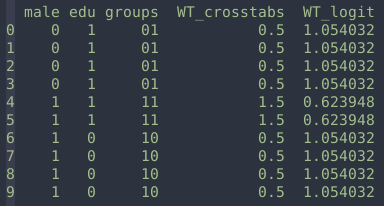
\includegraphics[width = 0.4\textwidth]  {figures/weight_logit_without_interaction.png}}
\label{fig:}
\end{figure}

You may find that the crosstabs weight and the logit weight are different! \\
{\textbf {Here is why:}}\\
\begin{itemize}
\item Crosstabs Weighting (Fully Saturated): This method treats every combination (e.g., Male + Edu) as a unique, independent island. It accounts for all interactions automatically. It doesn't care if "PhD" behaves similarly for Males and Females; it calculates them separately.
\item Logistic Regression (Additive): In a standard model (sample $ \sim  $ male + edu), the model assumes these variables are independent. It calculates a "bonus" for being Male and a "bonus" for having a PhD, then adds them together.
\item The Difference: If PhD holders are over-represented specifically among women but not among men, Crosstabs Weighting will catch that nuance. Logistic Regression will "average" the PhD effect across both genders unless you explicitly add an interaction term (e.g., male * edu).
\end{itemize}


{\textbf {Now include the interaction terms:}}

\begin{equation}
sample = \beta_0  +  \beta_1 male  + \beta_2 edu + \beta_3 male  \times edu.
\end{equation}
In python, you can set the equation as $ sample \sim male*edu $. It will include both the main
and the interaction effects.


Now the two weights are the same.
\begin{figure}[H]
\center{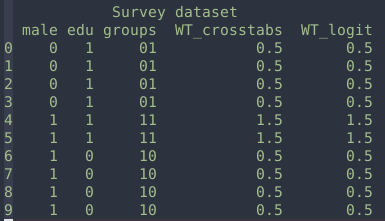
\includegraphics[width = 0.4\textwidth]  {figures/weight_logit_with_interaction.png}}
\label{fig:}
\end{figure}




\subsection{Advantage of logistic regression}
\begin{itemize}
\item It can include not only interaction terms, but multinomial terms, e.g., $ age^{2} $ .
\item It can handle continuous variable without creating intervals, such as age bins (21-25, 26-30).
\item Crosstabs groups may not be available for the population, and small cell sizes in the
		sample table.
\end{itemize}









\bibliographystyle{plainnat}
\bibliography{my_bib}

\end{document}

